%  Document History:
%
%-----------------------------------------------------------------------
\documentclass[a4paper,twoside]{arlims}
%------------------------------------------------------------------------- 

%--- Settings for the ARLIMS document class ---
\setcounter{page}{101} % The starting page

%--- This part of the preamble can be fiddled with according to our needs ---

% Some packages that we like and wan to use:
\usepackage{cite}
\usepackage{url}
\usepackage{graphicx}

% The path(s) to the graphics files:
\graphicspath{{eps/}{pdf/}}

% correct bad hyphenation here
\hyphenation{op-tical net-works semi-conduc-tor}

% This makes line breaks look prettier
\sloppy

%--- Preamble definitions for actual content ---

\title{Author Guidelines for Manuscripts}

%%% Only a single institute? Use the easy/proper way:
%
% \author{Your I. Name}
% \authorB{, An Othername}
% \authorC{ and Third Author}
% 
% \institute{Computer Science\\
% Institute of Information \& Mathematical Sciences\\
% Massey University at Albany, Auckland, New Zealand\\
% Email: \textnormal{\texttt{\{Y.I.Name | A.Othername | T.Author\}@massey.ac.nz}}}

%%% For authors in different institutes we need to trick a little more:

\author{Your I. Name}
\authorB{, An Othername}
\authorC[*]{ and Third Author}

\institute{
\begin{minipage}[t]{.45\textwidth}\centering
Institute of Information\\
\& Mathematical Sciences\\
Massey University at Albany,\\
Auckland, New Zealand\\
\textnormal{\texttt{\small\{Y.I.Name | A.Othername\}@massey.ac.nz}}
\end{minipage}}

\instituteB[]{
\begin{minipage}[t]{.45\textwidth}\centering
$^*$Encyclopedia Galactica, Research Division\\
Betelgeuse, Ursa Minor\\
\textnormal{\small\texttt{T.Author@encgal.edu}}
\end{minipage}}



%------------------------------------------------------------------------- 
\begin{document}

% Put a proper title on the first page:
\maketitle

%------------------------------------------------------------------------- 
\begin{abstract}
  The abstract is to be in fully-justified text, at the top as it is
  here, below the author information.  The abstract is to be in
  9-point, single-spaced type. Leave two blank lines after the
  abstract, then begin the main text. All manuscripts must be in
  English.
  
  \paragraph{Keywords:} small-worlds; computational Grid services; online
  communities; sparse matrices.
\end{abstract}

%------------------------------------------------------------------------- 
\section{Introduction}
\label{sect:Introduction}

These guidelines include complete descriptions of the fonts, spacing,
and related information for producing your proceedings manuscripts.
Please follow them and if you have any questions, direct them to the
editors in charge of the Research Letters.

\section{Formatting Your Paper}
\label{sect:Formatting}

All printed material, including text, illustrations, and charts, must
be kept within a print area of 15.0~cm wide by 22.7~cm high on A4
paper. Do not write or print anything outside the print area. Only the
title/volume title, the page numbers and the availability URL are to
appear after a 2.5~cm border from the top automatically.

The margins should be all properly aligned if the template is used.
All text must be in a one-column format and on A4 paper. Text must be
fully justified.

Please, make sure to avoid colour and colour figures if possible. The
document should be reproducible in black-and-white.


\subsection{Page Numbers/Margins on Odd Pages}
\label{sect:OddPageFormatting}

The binding margin (on the left) is to be 3.5~cm, and 2.5~cm on the
right hand side. The page header contains the paper title on the left
hand side, and the page number on the right hand side.


\subsection{Page Numbers/Margins on Even Pages}

The binding margin (on the right) is to be 3.5~cm, and 2.5~cm on the
left hand side. This is exactly the opposite of the odd side margins
as stated in Sect.~\ref{sect:OddPageFormatting}. The page header
contains the page number on the left hand side, and the authors on the
right hand side.


\subsection{Main Title}
\label{sect:MainTritle}

The main title (on the first page) should begin 5.0~cm from the top
edge of the page, centered, and in Times 14-point, boldface type.
Capitalize the first letter of nouns, pronouns, verbs, adjectives, and
adverbs; do not capitalize articles, coordinate conjunctions, or
prepositions (unless the title begins with such a word).  Leave a
blank line after the title.

\subsection{Author Name(s) and Affiliation(s)}
\label{sect:Authors}

Author names are to be centered beneath the title and printed in Times
12-point, non-boldface small capitals. Affiliations for multiple
authors may be shown in a two- or three-column format, with their
affiliations indicated. They are centered below the author names,
typeset in 10-point Times, italicized, not bold. Include e-mail
addresses if possible.  Follow the author information by a blank line
before main text.

\subsection{Second and Following Pages}
\label{sect:FollowingPages}

The second and following pages should begin 3.5~cm from the top edge.
On all pages, the bottom margin should be 3.5~cm from the bottom edge
of the page.

\subsection{Type-style and Fonts}
\label{sect:Fonts}

Wherever ``Times'' is specified, ``Times Roman'', or ``Times New
Roman'' may be used. If neither is available on your word processor,
please use the font closest in appearance to ``Times'' that you have
access to. Please avoid using bit-mapped fonts if possible. True-Type
or other high-quality \LaTeX\ fonts are preferred.

\subsection{Main Text}
\label{sect:MainText}

Type your main text in 10-point Times, single-spaced.  Do not use
double-spacing. All paragraphs (other than the first of a section)
should be indented 1 pica (approximately 0.4~cm). On the Microsoft
Word template make sure to use the style ``\texttt{Normal + First Line
  0 cm}'' for the sections' first paragraphs, and use
``\texttt{Normal}'' for the following ones. Be sure your text is fully
justified --- that is, flush left and flush right. Please do not place
any additional blank lines between paragraphs.

And this is a Table~\ref{tab:LINALG}, as you can see. Further
information on captioning of figures and tables is in the text below.

\begin{table*}[htbp]
  \caption{Linear Algebra Grid Services}
  \centering
  \begin{tabular}{|l|c|l|}
    \hline
    \textbf{Example Linear Algebra Services} & \textbf{Data Types} & \textbf{Resource Requirement} \\
    \hline
    Store a Matrix as part of a calculation  & M          &   Temp storage            \\
    Store a Vector as part of a calculation  & V          &   Temp storage            \\
    Store or retrieve a particular matrix    & M          &   Long term storage       \\
    Sparse Matrix to Dense Matrix Expand     & S: M       &   Compute + Temp Storage  \\
    Sparse Matrix Conjugate Gradient Solve   & S, V: V    &   Compute + Temp Storage  \\
    \hline
  \end{tabular}
  % Tables also like to have a label to be referenced ...
  \label{tab:LINALG}
\end{table*}

\textbf{Figure and table captions} should be 10-point Times,
non-boldface.  Callouts should be 9-point Times, non-boldface.
Initially capitalize only the first word of each figure caption and
table title. Figures and tables must be numbered separately. For
example: ``Figure 1.  Database contexts'', ``Table 1.  Input data''.
Figure captions are to be centered \emph{below} the figures. Table
titles are to be centered \emph{above} the tables.

And this is a Fig.~\ref{fig:timing}, as you can see ...

\begin{figure}[hbt]
  \centering
  % It is going to be 50% of the text's width and called "timing" ...
  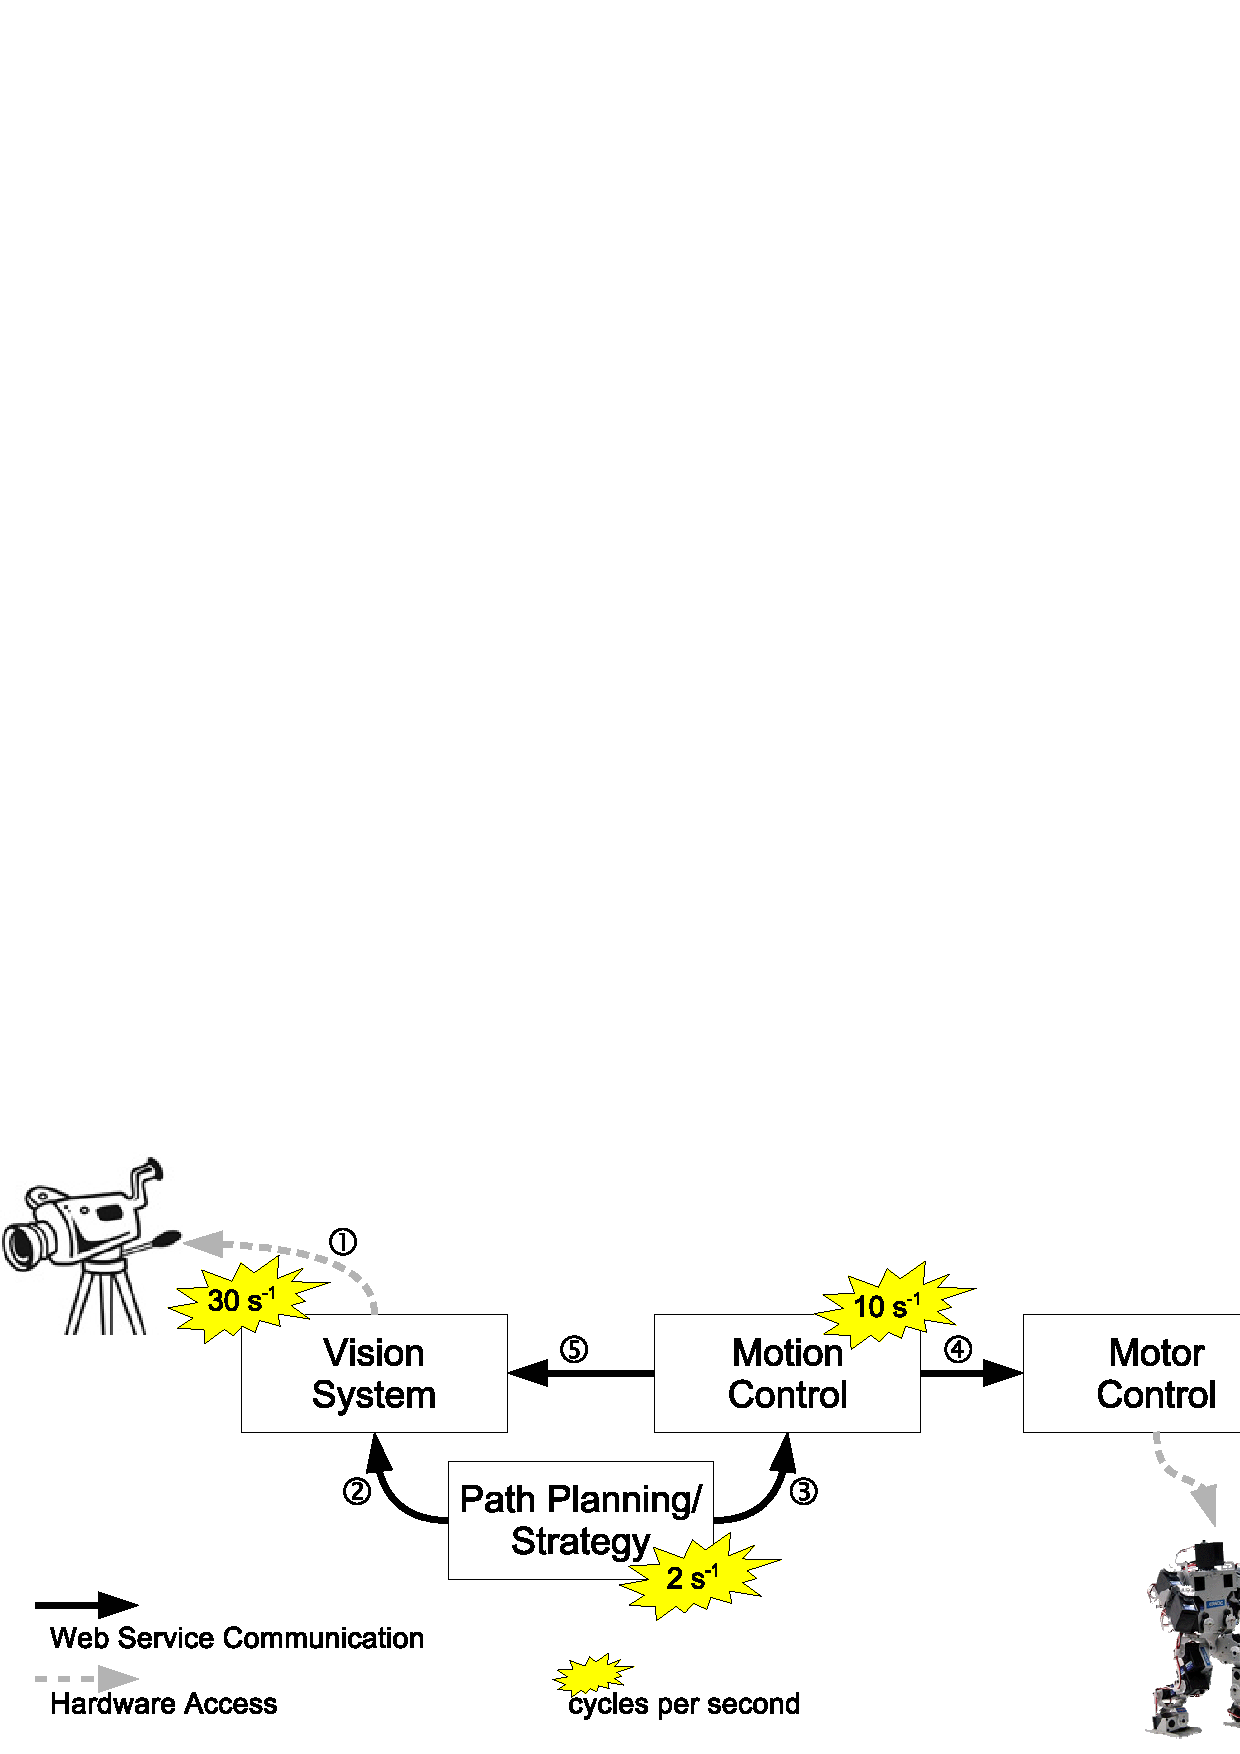
\includegraphics[width=.5\textwidth]{timing}
  \caption{Distribution of workflow components on the network.}
  % Look above, this is how we can reference it by a label ...
  \label{fig:timing}
\end{figure}

\section{First-Order Headings}
\label{sect:FirstOrderHeadings}

For example, ``1 Introduction'', should be Times 12-point boldface,
initially capitalized, flush left, with one blank line before, and one
blank line after. Do not use a period (``.'') after the heading
number.

\subsection{Second-Order Headings}
\label{sect:SecondOrderHeadings}

As in this heading, they should be Times 11-point boldface, initially
capitalized, flush left, with one blank line before, and one after.

\subsubsection{Third-Order Headings}
\label{sect:ThirdOrderHeadings}

Third-order headings, as in this paragraph, are discouraged. However,
if you must use them, use 10-point Times, boldface, initially
capitalized, flush left, with one blank line before, and one after.

\subsection{Footnotes}
\label{sect:Footnotes}

Use footnotes sparingly (or not at all!) and place them at the bottom
of the page on which they are referenced. Use Times 8-point type,
single-spaced. To help your readers, avoid using footnotes altogether
and include necessary peripheral observations in the text (within
parentheses, if you prefer, as in this sentence).

\subsection{References}
\label{sect:References}

List and number all bibliographical references in 10-point Times,
single-spaced, at the end of your paper.  When referenced in the text,
enclose the citation number in square brackets, for
example~\cite{FuzzyForCarLikeRobots}. Where appropriate, include the
name(s) of editors of referenced books. Several references should be
aggregated within the square
brackets~\cite{FuzzyForCarLikeRobots,other-reference}.

If you use Bib\TeX, please use the enclosed style
\texttt{IEEEtran.bst} (which is a slightly modified version of the
original \texttt{IEEEtran.bst}).

\subsection{Abbreviation of Words}
\label{sect:Abbreviations}

\begin{enumerate}
  \item The following should be abbreviated when they appear in
  running text unless they come at the beginning of a sentence: Chap.,
  Sect., Fig.; e.\,g.\ The results are depicted in Fig.~5. Figure~9
  reveals that \ldots

  \emph{Please note:} Equations should usually be referred to solely by their
  number in parentheses: e.\,g. (14).  However, when the reference
  comes at the beginning of a sentence, the unabbreviated word
  ``Equation'' should be used: e.\,g. Equation (14) is very important.
  However, (15) makes it clear that \ldots

  \item If abbreviations of names or concepts are used throughout the
  text, they should be defined at first occurrence, e.\,g.
  Plurisubharmonic (PSH) Functions, Strong Optimization (SOPT)
  Problem.
\end{enumerate}

\section{Copyright}
\label{sect:Copyright}

You retain the copyright of the material published in the RLIMS,
however you \emph{must} of course make sure that the material
published is \emph{not} covered under previous copyright restrictions.

%------------------------------------------------------------------------- 
\section*{Acknowledgements}

None in particular. But this section does not get numbered as it is
not part of the actual content.

%------------------------------------------------------------------------- 
%--- back matter: bibliography ---
% These are in alphabetical by leading author order.
\bibliographystyle{plain}
\begin{thebibliography}{10}

\bibitem{FuzzyForCarLikeRobots}
  A.~B. Foo, C.~D. Bar, and E.~F. Baz, ``{A Fuzzy Ergonomy Approach for
  Psycho-Spacial Distributed Sensor-Network Spaces,}''
  in \emph{Proceedings of the Third International Conference on
  Hot Wind Blowing in Academia}, Browns Bay, New Zealand, 2005.

\bibitem{other-reference}
  R. Barrett, M. Berry, et al.,
  ``Templates for the Solution of Linear Systems: Building Blocks for
  Iterative Methods,'' in \emph{SIAM,} Philadelphia, PA, 1994.

\end{thebibliography}

%%% If you want to use BibTeX, use the enclosed IEEEtran style:
% \bibliographystyle{IEEEtran}
% \bibliography{myreferences}

%------------------------------------------------------------------------- 
% We need this for the style to work properly, so please leave it in here:
\label{lastpagenum}
\end{document}
